% Options for packages loaded elsewhere
\PassOptionsToPackage{unicode}{hyperref}
\PassOptionsToPackage{hyphens}{url}
%
\documentclass[
]{article}
\usepackage{amsmath,amssymb}
\usepackage{lmodern}
\usepackage{ifxetex,ifluatex}
\ifnum 0\ifxetex 1\fi\ifluatex 1\fi=0 % if pdftex
  \usepackage[T1]{fontenc}
  \usepackage[utf8]{inputenc}
  \usepackage{textcomp} % provide euro and other symbols
\else % if luatex or xetex
  \usepackage{unicode-math}
  \defaultfontfeatures{Scale=MatchLowercase}
  \defaultfontfeatures[\rmfamily]{Ligatures=TeX,Scale=1}
\fi
% Use upquote if available, for straight quotes in verbatim environments
\IfFileExists{upquote.sty}{\usepackage{upquote}}{}
\IfFileExists{microtype.sty}{% use microtype if available
  \usepackage[]{microtype}
  \UseMicrotypeSet[protrusion]{basicmath} % disable protrusion for tt fonts
}{}
\makeatletter
\@ifundefined{KOMAClassName}{% if non-KOMA class
  \IfFileExists{parskip.sty}{%
    \usepackage{parskip}
  }{% else
    \setlength{\parindent}{0pt}
    \setlength{\parskip}{6pt plus 2pt minus 1pt}}
}{% if KOMA class
  \KOMAoptions{parskip=half}}
\makeatother
\usepackage{xcolor}
\IfFileExists{xurl.sty}{\usepackage{xurl}}{} % add URL line breaks if available
\IfFileExists{bookmark.sty}{\usepackage{bookmark}}{\usepackage{hyperref}}
\hypersetup{
  pdftitle={Tarea\_Est\_1},
  hidelinks,
  pdfcreator={LaTeX via pandoc}}
\urlstyle{same} % disable monospaced font for URLs
\usepackage[margin=1in]{geometry}
\usepackage{color}
\usepackage{fancyvrb}
\newcommand{\VerbBar}{|}
\newcommand{\VERB}{\Verb[commandchars=\\\{\}]}
\DefineVerbatimEnvironment{Highlighting}{Verbatim}{commandchars=\\\{\}}
% Add ',fontsize=\small' for more characters per line
\usepackage{framed}
\definecolor{shadecolor}{RGB}{248,248,248}
\newenvironment{Shaded}{\begin{snugshade}}{\end{snugshade}}
\newcommand{\AlertTok}[1]{\textcolor[rgb]{0.94,0.16,0.16}{#1}}
\newcommand{\AnnotationTok}[1]{\textcolor[rgb]{0.56,0.35,0.01}{\textbf{\textit{#1}}}}
\newcommand{\AttributeTok}[1]{\textcolor[rgb]{0.77,0.63,0.00}{#1}}
\newcommand{\BaseNTok}[1]{\textcolor[rgb]{0.00,0.00,0.81}{#1}}
\newcommand{\BuiltInTok}[1]{#1}
\newcommand{\CharTok}[1]{\textcolor[rgb]{0.31,0.60,0.02}{#1}}
\newcommand{\CommentTok}[1]{\textcolor[rgb]{0.56,0.35,0.01}{\textit{#1}}}
\newcommand{\CommentVarTok}[1]{\textcolor[rgb]{0.56,0.35,0.01}{\textbf{\textit{#1}}}}
\newcommand{\ConstantTok}[1]{\textcolor[rgb]{0.00,0.00,0.00}{#1}}
\newcommand{\ControlFlowTok}[1]{\textcolor[rgb]{0.13,0.29,0.53}{\textbf{#1}}}
\newcommand{\DataTypeTok}[1]{\textcolor[rgb]{0.13,0.29,0.53}{#1}}
\newcommand{\DecValTok}[1]{\textcolor[rgb]{0.00,0.00,0.81}{#1}}
\newcommand{\DocumentationTok}[1]{\textcolor[rgb]{0.56,0.35,0.01}{\textbf{\textit{#1}}}}
\newcommand{\ErrorTok}[1]{\textcolor[rgb]{0.64,0.00,0.00}{\textbf{#1}}}
\newcommand{\ExtensionTok}[1]{#1}
\newcommand{\FloatTok}[1]{\textcolor[rgb]{0.00,0.00,0.81}{#1}}
\newcommand{\FunctionTok}[1]{\textcolor[rgb]{0.00,0.00,0.00}{#1}}
\newcommand{\ImportTok}[1]{#1}
\newcommand{\InformationTok}[1]{\textcolor[rgb]{0.56,0.35,0.01}{\textbf{\textit{#1}}}}
\newcommand{\KeywordTok}[1]{\textcolor[rgb]{0.13,0.29,0.53}{\textbf{#1}}}
\newcommand{\NormalTok}[1]{#1}
\newcommand{\OperatorTok}[1]{\textcolor[rgb]{0.81,0.36,0.00}{\textbf{#1}}}
\newcommand{\OtherTok}[1]{\textcolor[rgb]{0.56,0.35,0.01}{#1}}
\newcommand{\PreprocessorTok}[1]{\textcolor[rgb]{0.56,0.35,0.01}{\textit{#1}}}
\newcommand{\RegionMarkerTok}[1]{#1}
\newcommand{\SpecialCharTok}[1]{\textcolor[rgb]{0.00,0.00,0.00}{#1}}
\newcommand{\SpecialStringTok}[1]{\textcolor[rgb]{0.31,0.60,0.02}{#1}}
\newcommand{\StringTok}[1]{\textcolor[rgb]{0.31,0.60,0.02}{#1}}
\newcommand{\VariableTok}[1]{\textcolor[rgb]{0.00,0.00,0.00}{#1}}
\newcommand{\VerbatimStringTok}[1]{\textcolor[rgb]{0.31,0.60,0.02}{#1}}
\newcommand{\WarningTok}[1]{\textcolor[rgb]{0.56,0.35,0.01}{\textbf{\textit{#1}}}}
\usepackage{graphicx}
\makeatletter
\def\maxwidth{\ifdim\Gin@nat@width>\linewidth\linewidth\else\Gin@nat@width\fi}
\def\maxheight{\ifdim\Gin@nat@height>\textheight\textheight\else\Gin@nat@height\fi}
\makeatother
% Scale images if necessary, so that they will not overflow the page
% margins by default, and it is still possible to overwrite the defaults
% using explicit options in \includegraphics[width, height, ...]{}
\setkeys{Gin}{width=\maxwidth,height=\maxheight,keepaspectratio}
% Set default figure placement to htbp
\makeatletter
\def\fps@figure{htbp}
\makeatother
\setlength{\emergencystretch}{3em} % prevent overfull lines
\providecommand{\tightlist}{%
  \setlength{\itemsep}{0pt}\setlength{\parskip}{0pt}}
\setcounter{secnumdepth}{-\maxdimen} % remove section numbering
\ifluatex
  \usepackage{selnolig}  % disable illegal ligatures
\fi

\title{Tarea\_Est\_1}
\author{}
\date{\vspace{-2.5em}}

\begin{document}
\maketitle

\hypertarget{pruebas-de-bondad-de-ajuste}{%
\subsection{Pruebas de bondad de
ajuste}\label{pruebas-de-bondad-de-ajuste}}

\hypertarget{problema-3}{%
\subsection{Problema 3}\label{problema-3}}

La siguiente muestra aleatoria hace referencia a los rendimientos
positivos de cierta acciC3n a lo largo del tiempo.

0.2513, 0.2566, 0.3459, 0.6379, 2.0505, 1.803, 2.1906, 1.5299, 0.35005,
0.3128, 1.2726, 2.3674, 2.3214, 2.4373, 0.6548

Llamamos a la libreria nortest para hacer la prueba lilliforce hasta el
final.

\begin{Shaded}
\begin{Highlighting}[]
\FunctionTok{library}\NormalTok{(nortest)}
\end{Highlighting}
\end{Shaded}

Ho: La muestra sigue una distribuciC3n normal VS Ha: La muestra no sigue
una distribuciC3n normal

Metemos los datos en un vector y ordenamos los datos.

\begin{Shaded}
\begin{Highlighting}[]
\NormalTok{Dirty\_data}\OtherTok{=}\FunctionTok{c}\NormalTok{(}\FloatTok{0.2513}\NormalTok{, }\FloatTok{0.2566}\NormalTok{, }\FloatTok{0.3459}\NormalTok{, }\FloatTok{0.6379}\NormalTok{, }\FloatTok{2.0505}\NormalTok{, }\FloatTok{1.803}\NormalTok{, }\FloatTok{2.1906}\NormalTok{,}
             \FloatTok{1.5299}\NormalTok{, }\FloatTok{0.35005}\NormalTok{, }\FloatTok{0.3128}\NormalTok{, }\FloatTok{1.2726}\NormalTok{, }\FloatTok{2.3674}\NormalTok{, }\FloatTok{2.3214}\NormalTok{, }\FloatTok{2.4373}\NormalTok{, }\FloatTok{0.6548}\NormalTok{)}
\NormalTok{Data}\OtherTok{=}\FunctionTok{sort}\NormalTok{(Dirty\_data)}
\end{Highlighting}
\end{Shaded}

\begin{verbatim}
##  [1] 0.25130 0.25660 0.31280 0.34590 0.35005 0.63790 0.65480 1.27260 1.52990
## [10] 1.80300 2.05050 2.19060 2.32140 2.36740 2.43730
\end{verbatim}

Como queremos probar normalidad pero no sabemos los parC!metros tenemos
que estimarlos, primero queremos hacer una funciC3n para calcular la
varianza muestral.

\begin{Shaded}
\begin{Highlighting}[]
\NormalTok{S2}\OtherTok{\textless{}{-}}\ControlFlowTok{function}\NormalTok{(x)\{}
\NormalTok{  mean\_aux}\OtherTok{=}\FunctionTok{mean}\NormalTok{(x)}
\NormalTok{  n\_aux}\OtherTok{=}\FunctionTok{length}\NormalTok{(x)}
\NormalTok{  s2}\OtherTok{=}\DecValTok{0}
  \ControlFlowTok{for}\NormalTok{ (i }\ControlFlowTok{in}\NormalTok{ x)\{}
\NormalTok{    s2}\OtherTok{=}\NormalTok{s2}\SpecialCharTok{+}\NormalTok{(i}\SpecialCharTok{{-}}\NormalTok{mean\_aux)}\SpecialCharTok{\^{}}\DecValTok{2}
\NormalTok{  \}}
\NormalTok{  s2}\OtherTok{=}\NormalTok{s2}\SpecialCharTok{/}\NormalTok{(n\_aux}\DecValTok{{-}1}\NormalTok{)}
  \FunctionTok{return}\NormalTok{(s2)}
\NormalTok{\}}
\end{Highlighting}
\end{Shaded}

Calculamos los estimadores mC!ximos verosC-miles.

\begin{Shaded}
\begin{Highlighting}[]
\NormalTok{mean\_est}\OtherTok{=}\FunctionTok{mean}\NormalTok{(Data)}
\NormalTok{S2\_est}\OtherTok{=}\FunctionTok{S2}\NormalTok{(Data)}
\NormalTok{n}\OtherTok{=}\FunctionTok{length}\NormalTok{(Data)}
\end{Highlighting}
\end{Shaded}

\begin{verbatim}
## [1] 1.252137
\end{verbatim}

\begin{verbatim}
## [1] 0.7810794
\end{verbatim}

\begin{verbatim}
## [1] 15
\end{verbatim}

Calculamos la funciC3n de distribuciC3n empC-rica necesaria para la
prueba de lillieforce, donde ``ecdf'' es la funciC3n para crear la
distribuciC3n empC-rica, ``f\_n'' son los percentiles de la
distribuciC3n empC-rica y ``f\_r'' son los percentiles de la
distribuciC3n pero desplazados una unidad.

\begin{Shaded}
\begin{Highlighting}[]
\NormalTok{f\_emp}\OtherTok{=}\FunctionTok{ecdf}\NormalTok{(Data)}
\NormalTok{f\_n}\OtherTok{=}\FunctionTok{f\_emp}\NormalTok{(Data)}
\NormalTok{f\_r}\OtherTok{=}\NormalTok{f\_n}\SpecialCharTok{{-}}\NormalTok{(}\DecValTok{1}\SpecialCharTok{/}\NormalTok{n) }
\end{Highlighting}
\end{Shaded}

Para para prueba de lillieforce necesitamos estandarizar los datos.

\begin{Shaded}
\begin{Highlighting}[]
\NormalTok{Z}\OtherTok{=}\NormalTok{(Data}\SpecialCharTok{{-}}\NormalTok{mean\_est)}\SpecialCharTok{/}\FunctionTok{sqrt}\NormalTok{(S2\_est)}
\end{Highlighting}
\end{Shaded}

\begin{verbatim}
##  [1] -1.13244110 -1.12644418 -1.06285419 -1.02540173 -1.02070603 -0.69500536
##  [7] -0.67588310  0.02315415  0.31428766  0.62329879  0.90334365  1.06186602
## [13]  1.20986549  1.26191423  1.34100569
\end{verbatim}

Ahora usaremos la funciC3n de distribuciC3n de una normal estandar para
los valores antes calculados.

\begin{Shaded}
\begin{Highlighting}[]
\NormalTok{Probas}\OtherTok{=}\FunctionTok{pnorm}\NormalTok{(Z)}
\end{Highlighting}
\end{Shaded}

\begin{verbatim}
##  [1] 0.1287245 0.1299888 0.1439240 0.1525868 0.1536969 0.2435260 0.2495574
##  [8] 0.5092363 0.6233487 0.7334559 0.8168282 0.8558517 0.8868347 0.8965102
## [15] 0.9100407
\end{verbatim}

Tenemos que calcular: \[ \frac{i}{n} - D_{i}^{+}=  \phi(Z_{i}) \]\\
\[D_{i}^{-}=  \phi(Z_{i}) - \frac{i-1}{n}\]

\begin{Shaded}
\begin{Highlighting}[]
\NormalTok{Di\_p}\OtherTok{=}\NormalTok{f\_n  }\SpecialCharTok{{-}}\NormalTok{Probas}
\NormalTok{Di\_n}\OtherTok{=}\NormalTok{ Probas }\SpecialCharTok{{-}}\NormalTok{ f\_r}
\end{Highlighting}
\end{Shaded}

Visualizamos todos los cC!lculos.

\begin{Shaded}
\begin{Highlighting}[]
\NormalTok{Visual}\OtherTok{=}\FunctionTok{data.frame}\NormalTok{(Dirty\_data,Data,Z,Probas,Di\_p,Di\_n)}
\end{Highlighting}
\end{Shaded}

\begin{verbatim}
##    Dirty_data    Data           Z    Probas         Di_p        Di_n
## 1     0.25130 0.25130 -1.13244110 0.1287245 -0.062057851  0.12872452
## 2     0.25660 0.25660 -1.12644418 0.1299888  0.003344555  0.06332211
## 3     0.34590 0.31280 -1.06285419 0.1439240  0.056075960  0.01059071
## 4     0.63790 0.34590 -1.02540173 0.1525868  0.114079830 -0.04741316
## 5     2.05050 0.35005 -1.02070603 0.1536969  0.179636464 -0.11296980
## 6     1.80300 0.63790 -0.69500536 0.2435260  0.156474028 -0.08980736
## 7     2.19060 0.65480 -0.67588310 0.2495574  0.217109233 -0.15044257
## 8     1.52990 1.27260  0.02315415 0.5092363  0.024096990  0.04256968
## 9     0.35005 1.52990  0.31428766 0.6233487 -0.023348715  0.09001538
## 10    0.31280 1.80300  0.62329879 0.7334559 -0.066789235  0.13345590
## 11    1.27260 2.05050  0.90334365 0.8168282 -0.083494899  0.15016157
## 12    2.36740 2.19060  1.06186602 0.8558517 -0.055851744  0.12251841
## 13    2.32140 2.32140  1.20986549 0.8868347 -0.020168078  0.08683474
## 14    2.43730 2.36740  1.26191423 0.8965102  0.036823158  0.02984351
## 15    0.65480 2.43730  1.34100569 0.9100407  0.089959302 -0.02329264
\end{verbatim}

Definimos \[D^{+}= max\{D_{i}^{+}\}\] \[D^{-}= max\{D_{i}^{-}\}\]

\begin{Shaded}
\begin{Highlighting}[]
\NormalTok{D\_p}\OtherTok{=}\FunctionTok{max}\NormalTok{(Di\_p)}
\NormalTok{D\_n}\OtherTok{=}\FunctionTok{max}\NormalTok{(Di\_n)}
\end{Highlighting}
\end{Shaded}

\begin{verbatim}
## [1] 0.2171092
\end{verbatim}

\begin{verbatim}
## [1] 0.1501616
\end{verbatim}

Definimos \[D= max\{ D^{+}, D^{-} \}\]

\begin{Shaded}
\begin{Highlighting}[]
\NormalTok{Dn}\OtherTok{=}\FunctionTok{max}\NormalTok{(D\_p,D\_n)}
\end{Highlighting}
\end{Shaded}

\begin{verbatim}
## [1] 0.2171092
\end{verbatim}

Declaramos nuestro nivel de significancia \[\alpha = 0.10\] entonces
\[1-\alpha = 0.90\].

Comparamos con el nivel crC-tico \[ W_{0.10}^{15}= 0.2016 \], para el
tamaC1o de muestra 15 en tablas.

\begin{Shaded}
\begin{Highlighting}[]
\NormalTok{Est}\OtherTok{=}\FloatTok{0.2016}
\NormalTok{Rechazamos\_H0}\OtherTok{=}\NormalTok{Dn}\SpecialCharTok{\textgreater{}}\NormalTok{Est}
\end{Highlighting}
\end{Shaded}

\begin{verbatim}
## [1] TRUE
\end{verbatim}

Como \[D > W_{0.10}^{15}\], rechazamos Ho y por lo tanto no hay
evidencia para que los datos sigan una distribuciC3n
\[ N(\mu,\sigma^2) \]

Hacemos la prueba en unas lC-neas.

\begin{Shaded}
\begin{Highlighting}[]
\NormalTok{p\_value}\OtherTok{=}\FunctionTok{lillie.test}\NormalTok{(Data)[[}\DecValTok{2}\NormalTok{]]}

\NormalTok{Rechazamos\_p\_value}\OtherTok{=}\NormalTok{p\_value}\SpecialCharTok{\textless{}}\NormalTok{alpha}
\end{Highlighting}
\end{Shaded}

\begin{verbatim}
## [1] 0.05540837
\end{verbatim}

\begin{verbatim}
## [1] TRUE
\end{verbatim}

Confirmando la prueba anterior.

El gerente del banco asume que la muestra se distribuye sigue una
distribuciC3n lognormal con media 0 y varianza 1. Realice la prueba
correspondiente para verificar la suposiciC3n del gerente con un nivel
de significancia alpha = 0.01.

Llamamos a la funciC3n de distribuciC3n de una lognormal.

\begin{Shaded}
\begin{Highlighting}[]
\NormalTok{ProbasB}\OtherTok{=}\FunctionTok{plnorm}\NormalTok{(Data) }
\end{Highlighting}
\end{Shaded}

\begin{verbatim}
##  [1] 0.0836229 0.0868775 0.1225789 0.1442074 0.1469328 0.3265089 0.3359924
##  [8] 0.5952465 0.6646554 0.7222209 0.7636471 0.7835314 0.8001537 0.8055991
## [15] 0.8135061
\end{verbatim}

Calculamos \$ D\_\{i\}\^{}\{+\}\$ y \$D\_\{i\}\^{}\{-\} \$

\begin{Shaded}
\begin{Highlighting}[]
\NormalTok{Di\_pB}\OtherTok{=}\FunctionTok{abs}\NormalTok{(ProbasB}\SpecialCharTok{{-}}\NormalTok{f\_n)}
\NormalTok{Di\_nB}\OtherTok{=}\FunctionTok{abs}\NormalTok{(ProbasB}\SpecialCharTok{{-}}\NormalTok{f\_r)}
\end{Highlighting}
\end{Shaded}

Ahora para \(D^{+} \quad D^{-}\)

\begin{Shaded}
\begin{Highlighting}[]
\NormalTok{D\_pB}\OtherTok{=}\FunctionTok{max}\NormalTok{(Di\_pB)}
\CommentTok{\#Calculamos D{-}}
\NormalTok{D\_nB}\OtherTok{=}\FunctionTok{max}\NormalTok{(Di\_nB)}
\end{Highlighting}
\end{Shaded}

Entonces obtenemos \(D\)

\begin{Shaded}
\begin{Highlighting}[]
\NormalTok{DnB}\OtherTok{=}\FunctionTok{max}\NormalTok{(D\_pB,D\_nB)}
\end{Highlighting}
\end{Shaded}

\begin{verbatim}
## [1] 0.1864939
\end{verbatim}

Declaramos nuestro nivel de significancia \[\alpha = 0.01\] entonces
\[1-\alpha = 0.99\].

Tenemos que en tablas \[W_{0.01}^{15}=0.40420\]

\begin{Shaded}
\begin{Highlighting}[]
\NormalTok{EstB}\OtherTok{=}\FloatTok{0.40420}

\NormalTok{Rechazamos\_H0B}\OtherTok{=}\NormalTok{DnB}\SpecialCharTok{\textgreater{}}\NormalTok{EstB}
\end{Highlighting}
\end{Shaded}

\begin{verbatim}
## [1] FALSE
\end{verbatim}

Se cumple que \[W_{0.01}^{15} > D\] entonces no hay evidencia para
rechazar Ho, entonces los datos siguen una distribuciC3n lognormal con
media de 1 y varianza 0.

Usamos la prueba especC-ficando la distribuciC3n lognormal con sus
parC!metros.

\begin{Shaded}
\begin{Highlighting}[]
\NormalTok{p\_valueB}\OtherTok{=}\FunctionTok{ks.test}\NormalTok{(Data,plnorm,}\DecValTok{0}\NormalTok{,}\DecValTok{1}\NormalTok{)[[}\DecValTok{2}\NormalTok{]]}

\NormalTok{Rechazamos\_p\_valueB}\OtherTok{=}\NormalTok{p\_valueB}\SpecialCharTok{\textless{}}\NormalTok{alphaB}
\end{Highlighting}
\end{Shaded}

\begin{verbatim}
## [1] 0.6089758
\end{verbatim}

\begin{verbatim}
## [1] FALSE
\end{verbatim}

Confirmamos la prueba anterior.

\hypertarget{pruebas-de-bondad-de-ajuste-1}{%
\subsection{Pruebas de bondad de
ajuste}\label{pruebas-de-bondad-de-ajuste-1}}

\hypertarget{problema-4}{%
\subsection{Problema 4}\label{problema-4}}

Un cierto banco otorga crC)dito a las personas con una tasa
preferencial, de tal manera que los acreditados pueden pagar en
cualquier momento desde que piden el prestamo hasta 8 semanas
posteriores para que les sea respetada la tasa preferencial . Se
seleccionaron aleatoriamente a 1,000 personas y observaron su
comportamiento, generando de esta manera la siguiente tabla de
frecuencia:

\begin{Shaded}
\begin{Highlighting}[]
\NormalTok{intervalos }\OtherTok{\textless{}{-}} \FunctionTok{c}\NormalTok{( }\StringTok{"Menos de 1 semana"}\NormalTok{,}\StringTok{"1\textless{}= x \textless{}2"}\NormalTok{ , }\StringTok{"2\textless{}= x \textless{}3"}\NormalTok{,}\StringTok{"3\textless{}= x \textless{}4"}\NormalTok{,}\StringTok{"4\textless{}= x \textless{}5"}\NormalTok{,}\StringTok{"5\textless{}= x \textless{}6"}\NormalTok{,}\StringTok{"6\textless{}= x \textless{}7"}\NormalTok{,}\StringTok{"7\textless{}= x \textless{}8"}\NormalTok{,}\StringTok{"MC!s de 8 semanas"}\NormalTok{)}
\NormalTok{oi }\OtherTok{\textless{}{-}} \FunctionTok{c}\NormalTok{(}\DecValTok{64}\NormalTok{,}\DecValTok{195}\NormalTok{,}\DecValTok{287}\NormalTok{,}\DecValTok{241}\NormalTok{,}\DecValTok{140}\NormalTok{,}\DecValTok{51}\NormalTok{,}\DecValTok{25}\NormalTok{,}\DecValTok{4}\NormalTok{,}\DecValTok{1}\NormalTok{)}

\NormalTok{tabla }\OtherTok{\textless{}{-}} \FunctionTok{data.frame}\NormalTok{(oi,}\AttributeTok{row.names =}\NormalTok{ intervalos )}
\NormalTok{tabla}
\end{Highlighting}
\end{Shaded}

\begin{verbatim}
##                    oi
## Menos de 1 semana  64
## 1<= x <2          195
## 2<= x <3          287
## 3<= x <4          241
## 4<= x <5          140
## 5<= x <6           51
## 6<= x <7           25
## 7<= x <8            4
## MC!s de 8 semanas   1
\end{verbatim}

Observamos la cantidad real de personas.

\begin{Shaded}
\begin{Highlighting}[]
\NormalTok{k}\OtherTok{=}\FunctionTok{sum}\NormalTok{(oi)}
\FunctionTok{print}\NormalTok{(k)}
\end{Highlighting}
\end{Shaded}

\begin{verbatim}
## [1] 1008
\end{verbatim}

Sea X v.a. que modela semanas completas que se tarda el cliente en hacer
el pago.

Enunciamos la prueba de hipC3tesis:

Ho: Se sigue una distribuciC3n Bin(n=10,p=0.25) VS Ha: No se sigue una
distribuciC3n Bin(n=10,p=0.25)

Nuestros parC!metros son:

\begin{Shaded}
\begin{Highlighting}[]
\NormalTok{p}\OtherTok{=}\FloatTok{0.25}
\NormalTok{n}\OtherTok{=}\DecValTok{10}
\end{Highlighting}
\end{Shaded}

Los datos se agruparon en nueve diferentes clasificaciones
\(c_{i} \quad i\in \{0,1,...,8 \}\).

\begin{Shaded}
\begin{Highlighting}[]
\FunctionTok{length}\NormalTok{(oi)}
\end{Highlighting}
\end{Shaded}

\begin{verbatim}
## [1] 9
\end{verbatim}

Nuestras observaciones fueron:

\begin{Shaded}
\begin{Highlighting}[]
\NormalTok{oi}\OtherTok{=}\FunctionTok{c}\NormalTok{(}\DecValTok{64}\NormalTok{,}\DecValTok{195}\NormalTok{,}\DecValTok{287}\NormalTok{,}\DecValTok{241}\NormalTok{,}\DecValTok{140}\NormalTok{,}\DecValTok{51}\NormalTok{,}\DecValTok{25}\NormalTok{,}\DecValTok{4}\NormalTok{,}\DecValTok{1}\NormalTok{)}
\end{Highlighting}
\end{Shaded}

Calculamos las probabilidades \(p_{i}\) con la distribuciC3n que
propusimos, se itera desde cero ya que tenemos la clasificaciC3n 0.

\begin{verbatim}
## [1] 0.056313515 0.187711716 0.281567574 0.250282288 0.145998001 0.058399200
## [7] 0.016222000 0.003089905 0.000415802
\end{verbatim}

Verificamos que las probas suman 1. \[\sum_{i=0}^{8} p_{i} = 1\]

\begin{Shaded}
\begin{Highlighting}[]
\FunctionTok{sum}\NormalTok{(Probas\_ejercicio4)}
\end{Highlighting}
\end{Shaded}

\begin{verbatim}
## [1] 1
\end{verbatim}

Ahora calculamos las frecuencias esperadas.

\[n * p_{i}\]

\begin{Shaded}
\begin{Highlighting}[]
\NormalTok{ei}\OtherTok{=}\NormalTok{ Probas\_ejercicio4 }\SpecialCharTok{*}\NormalTok{ k }
\FunctionTok{print}\NormalTok{(ei)}
\end{Highlighting}
\end{Shaded}

\begin{verbatim}
## [1]  56.7640228 189.2134094 283.8201141 252.2845459 147.1659851  58.8663940
## [7]  16.3517761   3.1146240   0.4191284
\end{verbatim}

Podemos visualizar toda la informaciC3n.

\begin{Shaded}
\begin{Highlighting}[]
\NormalTok{Tabla\_ji }\OtherTok{=} \FunctionTok{data.frame}\NormalTok{(}\StringTok{"ci"}\OtherTok{=}\DecValTok{0}\SpecialCharTok{:}\DecValTok{8}\NormalTok{, }\StringTok{"oi"}\OtherTok{=}\NormalTok{oi,}\StringTok{"pi"}\OtherTok{=}\NormalTok{ Probas\_ejercicio4,}\StringTok{"ei"}\OtherTok{=}\NormalTok{ei)}
\FunctionTok{print}\NormalTok{(Tabla\_ji)}
\end{Highlighting}
\end{Shaded}

\begin{verbatim}
##   ci  oi          pi          ei
## 1  0  64 0.056313515  56.7640228
## 2  1 195 0.187711716 189.2134094
## 3  2 287 0.281567574 283.8201141
## 4  3 241 0.250282288 252.2845459
## 5  4 140 0.145998001 147.1659851
## 6  5  51 0.058399200  58.8663940
## 7  6  25 0.016222000  16.3517761
## 8  7   4 0.003089905   3.1146240
## 9  8   1 0.000415802   0.4191284
\end{verbatim}

Vamos a calcular nuestra estadC-stica de prueba.
\[T= \sum _{i=0}^{8} \frac{(o_{i}-e_{i})^{2}}{e_{i}}\]

\begin{Shaded}
\begin{Highlighting}[]
\NormalTok{EstJi}\OtherTok{=}\DecValTok{0} 
\ControlFlowTok{for}\NormalTok{ (i }\ControlFlowTok{in} \DecValTok{1}\SpecialCharTok{:}\DecValTok{9}\NormalTok{)\{}
\NormalTok{  EstJi}\OtherTok{=}\NormalTok{EstJi}\SpecialCharTok{+}\NormalTok{(((oi[i]) }\SpecialCharTok{{-}}\NormalTok{ (ei[i]))}\SpecialCharTok{\^{}}\DecValTok{2}\NormalTok{)}\SpecialCharTok{/}\NormalTok{(ei[i])}
\NormalTok{\}}
\FunctionTok{print}\NormalTok{(EstJi)}
\end{Highlighting}
\end{Shaded}

\begin{verbatim}
## [1] 8.670518
\end{verbatim}

Se comienza el ciclo desde 1 hasta 9 ya que son las entradas de los
vectores, no son las clasificaciones.

Para un nivel de confianza \$\alpha = 0.01 \$ tenemos que
\(1-\alpha = 0.99\).

\begin{Shaded}
\begin{Highlighting}[]
\NormalTok{alpha\_ejercicio4}\OtherTok{=}\FloatTok{0.01}
\NormalTok{conf\_ejercicio4}\OtherTok{=} \DecValTok{1}\SpecialCharTok{{-}}\NormalTok{ alpha\_ejercicio4}
\end{Highlighting}
\end{Shaded}

Necesitamos los grados de libertad, que es el nC:mero de clasificaciones
menos uno, ya que no estimamos parC!metros.

\begin{verbatim}
## [1] 8
\end{verbatim}

Calculamos el cuantil \({\chi}^2_{8,\ 0.99}\).

\begin{Shaded}
\begin{Highlighting}[]
\NormalTok{valor\_critico}\OtherTok{=}\FunctionTok{qchisq}\NormalTok{(conf\_ejercicio4,}\AttributeTok{df=}\NormalTok{v,}\AttributeTok{lower.tail =} \ConstantTok{TRUE}\NormalTok{)}
\end{Highlighting}
\end{Shaded}

Comparamos la estadC-stica de prueba con el valor crC-tico.

\begin{Shaded}
\begin{Highlighting}[]
\NormalTok{Rechazamos\_H0\_p4}\OtherTok{=}\NormalTok{EstJi}\SpecialCharTok{\textgreater{}}\NormalTok{valor\_critico}
\FunctionTok{print}\NormalTok{(Rechazamos\_H0\_p4)}
\end{Highlighting}
\end{Shaded}

\begin{verbatim}
## [1] FALSE
\end{verbatim}

No hay evidencia pra decir que los datos no siguien una distribuciC3n
binomial con n=10 y p=0.25, entonces aceptamos Ho.

Para comprobar los cC!lculos usemos la prueba que vienen en la libreria
nortest.

\begin{Shaded}
\begin{Highlighting}[]
\NormalTok{p\_value\_p4}\OtherTok{=}\FunctionTok{chisq.test}\NormalTok{(}\AttributeTok{x=}\NormalTok{oi,}\AttributeTok{p=}\NormalTok{Probas\_ejercicio4)[[}\DecValTok{3}\NormalTok{]]}
\end{Highlighting}
\end{Shaded}

\begin{verbatim}
## Warning in chisq.test(x = oi, p = Probas_ejercicio4): Chi-squared approximation
## may be incorrect
\end{verbatim}

\begin{Shaded}
\begin{Highlighting}[]
\NormalTok{Rechazamos\_p\_value\_p4}\OtherTok{=}\NormalTok{alpha\_ejercicio4}\SpecialCharTok{\textgreater{}}\NormalTok{p\_value\_p4}
\FunctionTok{print}\NormalTok{(Rechazamos\_p\_value\_p4)}
\end{Highlighting}
\end{Shaded}

\begin{verbatim}
## [1] FALSE
\end{verbatim}

No rechazamos Ho.

\hypertarget{pruebas-de-bondad-de-ajuste-2}{%
\subsection{Pruebas de bondad de
ajuste}\label{pruebas-de-bondad-de-ajuste-2}}

\hypertarget{problema-5}{%
\subsection{Problema 5}\label{problema-5}}

En R fije la semilla 2019, y genera 25 observaciones distribuidas como
una N(0; 1) y con ella realiza:

Calcula y grC!fica la funciC3n de distribuciC3n empC-rica de las
observaciones generadas.

Agrega sobre esa misma grC!fica, la curva de la distribuciC3n verdadera
(N(0; 1)). A partir de las grC!ficas anteriores B?La funciC3n de
distribuciC3n empC-rica es similar a la distribucin teC3rica de los
datos?.

Vuelve a fijar la semilla 2019, y genera un millC3n de observaciones
distribuidas como una N(0; 1) y con ello realiza:

Calcula y grC!fica la funciC3n de distribuciC3n empC-rica de las
observaciones generadas.

Agrega sobre esa misma grC!fica, la curva de la distribuciC3n verdadera
(N(0; 1)). A partir de las grC!ficas anteriores B?La funciC3n de
distribuciC3n empC-rica es similar a la distribuciC3n teC3rica de los
datos?.

Realiza la diferencia entre el valor de la funciC3n empC-rica y la
funciC3n real, (Hint: no olvides que debes ordenar de menor a mayor los
valores de la distribuciC3n conocida y sC3lo mostrar los primeros 5 y
los C:ltimos 5 resultados)

B?Al ser una muestra mucho mayor que al anterior a que teorema te
recuerda el resultado obtenido?.

Para la primera parte del ejercicio fijemos la semilla inicial.

\begin{Shaded}
\begin{Highlighting}[]
\FunctionTok{set.seed}\NormalTok{(}\DecValTok{2019}\NormalTok{)}
\end{Highlighting}
\end{Shaded}

Obtengamos 25 datos de una distribuciC3n normal estC!ndar.

\begin{Shaded}
\begin{Highlighting}[]
\NormalTok{x\_data}\OtherTok{=}\FunctionTok{rnorm}\NormalTok{(}\DecValTok{25}\NormalTok{,}\AttributeTok{mean=}\DecValTok{0}\NormalTok{,}\AttributeTok{sd=}\DecValTok{1}\NormalTok{)}
\FunctionTok{print}\NormalTok{(x\_data)}
\end{Highlighting}
\end{Shaded}

\begin{verbatim}
##  [1]  0.7385227 -0.5147605 -1.6401813  0.9160368 -1.2674820  0.7382478
##  [7] -0.7826228  0.5092959 -1.4899391 -0.3191793 -0.2379111  1.6186229
## [13] -1.1176011  0.2340028  0.3161516  0.3707686  0.8775886 -1.7683235
## [19] -0.3271264 -2.2632252  0.2855605  0.9684286  0.8673066  1.3781350
## [25] -0.8082596
\end{verbatim}

Calculemos la funciC3n de distribuciC3n empC-rica y obtengamos su
grC!fica.

\begin{Shaded}
\begin{Highlighting}[]
\NormalTok{f\_empi}\OtherTok{=}\FunctionTok{ecdf}\NormalTok{(x\_data)}
\FunctionTok{plot}\NormalTok{(f\_empi, }\AttributeTok{xlab=}\StringTok{"Observados"}\NormalTok{, }\AttributeTok{ylab=}\StringTok{"FunciC3n de probabilidad"}\NormalTok{, }
     \AttributeTok{main=}\StringTok{"Muestra con 25 valores"}\NormalTok{, }\AttributeTok{col=}\StringTok{"darkcyan"}\NormalTok{)}
\FunctionTok{curve}\NormalTok{(}\FunctionTok{pnorm}\NormalTok{(x), }\AttributeTok{add=}\ConstantTok{TRUE}\NormalTok{, }\AttributeTok{col=}\StringTok{"red"}\NormalTok{)}
\end{Highlighting}
\end{Shaded}

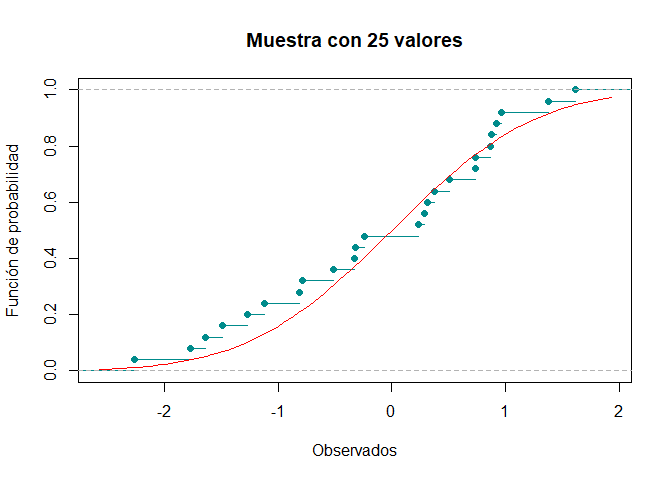
\includegraphics{Pruebas_p_files/figure-html/unnamed-chunk-52-1.png}

Las funciones se parecen aunque pareciera que el error el algo grande ya
que no son idC)nticas, del lado de los negativos se aprecia mC!s
despegada en cambio para valores mayores a cero se ajustan mejor a la
funciC3n de distribuciC3n de una \(N(0,1)\).

Vamos con la segunda parte del ejercicio, primero volvemos a fijar la
semilla.

\begin{Shaded}
\begin{Highlighting}[]
\FunctionTok{set.seed}\NormalTok{(}\DecValTok{2019}\NormalTok{)}
\end{Highlighting}
\end{Shaded}

Generamos un millC3n de datos de una distribuciC3n \(N(0,1)\).

\begin{Shaded}
\begin{Highlighting}[]
\NormalTok{x\_dataM }\OtherTok{=} \FunctionTok{rnorm}\NormalTok{(}\DecValTok{10}\SpecialCharTok{\^{}}\DecValTok{3}\NormalTok{)}
\end{Highlighting}
\end{Shaded}

Calculamos la funciC3n de distribuciC3n empC-rica \(F_{n}\)

\begin{Shaded}
\begin{Highlighting}[]
\NormalTok{f\_empiM }\OtherTok{=} \FunctionTok{ecdf}\NormalTok{(x\_dataM)}
\end{Highlighting}
\end{Shaded}

Veamos las grC!ficas:

\begin{Shaded}
\begin{Highlighting}[]
\FunctionTok{plot}\NormalTok{(f\_empiM, }\AttributeTok{xlab=}\StringTok{"Observados"}\NormalTok{, }\AttributeTok{ylab=}\StringTok{"FunciC3n de probabilidad"}\NormalTok{, }
     \AttributeTok{main=}\StringTok{"Muestra con 10\^{}6 valores"}\NormalTok{, }\AttributeTok{col=}\StringTok{"darkcyan"}\NormalTok{)}
\FunctionTok{curve}\NormalTok{(}\FunctionTok{pnorm}\NormalTok{(x), }\AttributeTok{add=}\ConstantTok{TRUE}\NormalTok{, }\AttributeTok{col=}\StringTok{"red"}\NormalTok{)}
\end{Highlighting}
\end{Shaded}

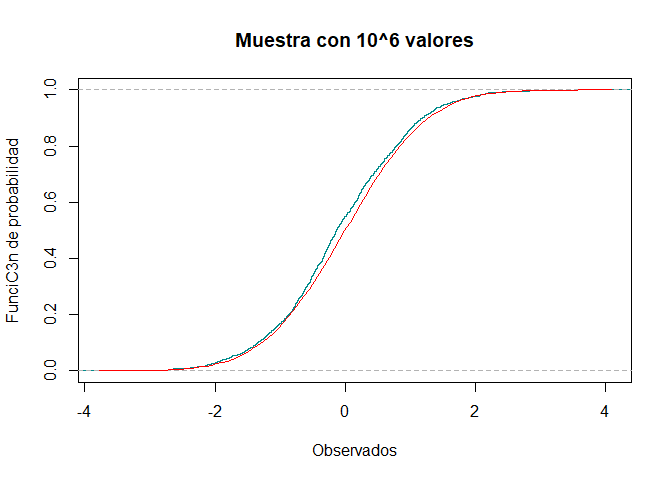
\includegraphics{Pruebas_p_files/figure-html/unnamed-chunk-56-1.png}

En este caso para una muestra de tamaC1o \(10^6\), ambas funciones se
parecen mucho, apenas se alcanzan a ver los puntos en los que difieren.

Trabajemos con la muestra tamaC1o 25, ahora vamos a ver como se
comportan los datos en relaciC3n con la funciC3n empC-rica y real,
primero debemos ordenar los datos.

\begin{Shaded}
\begin{Highlighting}[]
\NormalTok{x\_data\_ord}\OtherTok{=}\FunctionTok{sort}\NormalTok{(x\_data)}
\NormalTok{f\_empi\_norm}\OtherTok{=}\FunctionTok{f\_empi}\NormalTok{(x\_data\_ord)}
\end{Highlighting}
\end{Shaded}

Calculemos la funciC3n empC-rica con un lugar desfasado (salto de
\(\frac{1}{25}\)).

\begin{Shaded}
\begin{Highlighting}[]
\NormalTok{f\_empi\_des}\OtherTok{=}\NormalTok{f\_empi\_norm }\SpecialCharTok{{-}}\NormalTok{ (}\DecValTok{1}\SpecialCharTok{/}\DecValTok{25}\NormalTok{)}
\end{Highlighting}
\end{Shaded}

Calculemos las probabilidades de la muestra suponiendo una distribuciC3n
\(N(0,1)\).

\begin{Shaded}
\begin{Highlighting}[]
\NormalTok{probras\_data }\OtherTok{=} \FunctionTok{pnorm}\NormalTok{(x\_data\_ord)}
\end{Highlighting}
\end{Shaded}

Primero vamos con \(D^{+}\).

\begin{Shaded}
\begin{Highlighting}[]
\NormalTok{D\_data\_norm }\OtherTok{=}\NormalTok{ f\_empi\_norm }\SpecialCharTok{{-}}\NormalTok{ probras\_data}
\NormalTok{D\_data\_max }\OtherTok{=} \FunctionTok{max}\NormalTok{(D\_data\_norm)}
\FunctionTok{print}\NormalTok{(D\_data\_max)}
\end{Highlighting}
\end{Shaded}

\begin{verbatim}
## [1] 0.1081313
\end{verbatim}

Ahora para \(D^{-}\)

\begin{Shaded}
\begin{Highlighting}[]
\NormalTok{D\_data\_des }\OtherTok{=}\NormalTok{ probras\_data }\SpecialCharTok{{-}}\NormalTok{ f\_empi\_des}
\NormalTok{D\_data\_des\_max }\OtherTok{=} \FunctionTok{max}\NormalTok{(D\_data\_des)}
\FunctionTok{print}\NormalTok{(D\_data\_des\_max)}
\end{Highlighting}
\end{Shaded}

\begin{verbatim}
## [1] 0.1125086
\end{verbatim}

Ahora calculamos \(D = max \{D^{+},D^{-} \}= \sup |F_{n}(x) - F(x) |\),
que es la diferencia entre la funciC3n de distribuciC3n empC-rica y
teC3rica, al final vamos a comparar con la de la simulaciC3n \(10^{6}\).

\begin{Shaded}
\begin{Highlighting}[]
\NormalTok{D\_max}\OtherTok{=} \FunctionTok{max}\NormalTok{(D\_data\_max,D\_data\_des\_max)}
\FunctionTok{print}\NormalTok{(D\_max)}
\end{Highlighting}
\end{Shaded}

\begin{verbatim}
## [1] 0.1125086
\end{verbatim}

Veamos la informaciCiC3n:

Mostremos los 5 primeros datos y C:ltimos 5:

\begin{Shaded}
\begin{Highlighting}[]
\FunctionTok{print}\NormalTok{(}\FunctionTok{head}\NormalTok{(valores\_25))}
\end{Highlighting}
\end{Shaded}

\begin{verbatim}
##       x_data x_data_ord probras_data D_data_norm   D_data_des
## 1  0.7385227  -2.263225   0.01181090  0.02818910  0.011810905
## 2 -0.5147605  -1.768324   0.03850342  0.04149658 -0.001496583
## 3 -1.6401813  -1.640181   0.05048373  0.06951627 -0.029516266
## 4  0.9160368  -1.489939   0.06812013  0.09187987 -0.051879873
## 5 -1.2674820  -1.267482   0.10249150  0.09750850 -0.057508497
## 6  0.7382478  -1.117601   0.13186870  0.10813130 -0.068131302
\end{verbatim}

\begin{Shaded}
\begin{Highlighting}[]
\FunctionTok{print}\NormalTok{(}\FunctionTok{tail}\NormalTok{(valores\_25))}
\end{Highlighting}
\end{Shaded}

\begin{verbatim}
##        x_data x_data_ord probras_data  D_data_norm   D_data_des
## 20 -2.2632252  0.8673066    0.8071130 -0.007112981  0.047112981
## 21  0.2855605  0.8775886    0.8099165  0.030083517  0.009916483
## 22  0.9684286  0.9160368    0.8201762  0.059823801 -0.019823801
## 23  0.8673066  0.9684286    0.8335848  0.086415187 -0.046415187
## 24  1.3781350  1.3781350    0.9159192  0.044080808 -0.004080808
## 25 -0.8082596  1.6186229    0.9472358  0.052764213 -0.012764213
\end{verbatim}

Vamos a hacer lo mismo para los datos de la simulaciC3n \(10^{6}\), y
despuC)s vamos comparar las \(D\). Ordenamos la muestra.

\begin{Shaded}
\begin{Highlighting}[]
\NormalTok{x\_dataM\_ord }\OtherTok{=} \FunctionTok{sort}\NormalTok{(x\_dataM)}
\NormalTok{f\_empi\_M}\OtherTok{=} \FunctionTok{f\_empiM}\NormalTok{(x\_dataM\_ord)}
\end{Highlighting}
\end{Shaded}

Calculamos la funciciC3n desfasada (\(\frac{1}{10^6}\)).

\begin{Shaded}
\begin{Highlighting}[]
\NormalTok{f\_empi\_M\_des }\OtherTok{=}\NormalTok{ f\_empi\_M }\SpecialCharTok{{-}}\NormalTok{ (}\DecValTok{1}\SpecialCharTok{/}\NormalTok{(}\DecValTok{10}\SpecialCharTok{\^{}}\DecValTok{3}\NormalTok{))}
\end{Highlighting}
\end{Shaded}

Calculamos las probas bajo una distribuciones \(N(0,1)\).

\begin{Shaded}
\begin{Highlighting}[]
\NormalTok{probas\_dataM }\OtherTok{=} \FunctionTok{pnorm}\NormalTok{(x\_dataM\_ord)}
\end{Highlighting}
\end{Shaded}

Calculamos \(D^{+}=\max \{F_{n}(x_{i}) - F(x_{i}) \}\).

\begin{Shaded}
\begin{Highlighting}[]
\NormalTok{D\_dataM\_norm }\OtherTok{=}\NormalTok{ f\_empi\_M }\SpecialCharTok{{-}}\NormalTok{ probas\_dataM}
\NormalTok{D\_dataM\_norm\_max }\OtherTok{=} \FunctionTok{max}\NormalTok{(D\_dataM\_norm)}
\FunctionTok{print}\NormalTok{(D\_dataM\_norm\_max)}
\end{Highlighting}
\end{Shaded}

\begin{verbatim}
## [1] 0.05626327
\end{verbatim}

Calculamos \(D^{-}=\max \{F(x_{i}) - F_{n}(x_{i-1}) \}\).

\begin{Shaded}
\begin{Highlighting}[]
\NormalTok{D\_dataM\_des }\OtherTok{=}\NormalTok{ probas\_dataM }\SpecialCharTok{{-}}\NormalTok{ f\_empi\_M\_des}
\NormalTok{D\_dataM\_des\_max }\OtherTok{=} \FunctionTok{max}\NormalTok{(D\_dataM\_des)}
\FunctionTok{print}\NormalTok{(D\_data\_des\_max)}
\end{Highlighting}
\end{Shaded}

\begin{verbatim}
## [1] 0.1125086
\end{verbatim}

Ahora calculamos \(D\).

\begin{Shaded}
\begin{Highlighting}[]
\NormalTok{D\_maxM }\OtherTok{=} \FunctionTok{max}\NormalTok{(D\_dataM\_norm\_max, D\_data\_des\_max)}
\FunctionTok{print}\NormalTok{(D\_data\_des\_max)}
\end{Highlighting}
\end{Shaded}

\begin{verbatim}
## [1] 0.1125086
\end{verbatim}

Mostremos los 5 primeros datos y C:ltimos 5:

\begin{Shaded}
\begin{Highlighting}[]
\FunctionTok{print}\NormalTok{(}\FunctionTok{head}\NormalTok{(valores\_M))}
\end{Highlighting}
\end{Shaded}

\begin{verbatim}
##      x_dataM x_dataM_ord probas_dataM D_dataM_norm   D_dataM_des
## 1  0.7385227   -3.236082 0.0006059136 0.0003940864  0.0006059136
## 2 -0.5147605   -3.186318 0.0007204796 0.0012795204 -0.0002795204
## 3 -1.6401813   -3.096515 0.0009790485 0.0020209515 -0.0010209515
## 4  0.9160368   -2.699617 0.0034709701 0.0005290299  0.0004709701
## 5 -1.2674820   -2.693624 0.0035339936 0.0014660064 -0.0004660064
## 6  0.7382478   -2.665872 0.0038394508 0.0021605492 -0.0011605492
\end{verbatim}

\begin{Shaded}
\begin{Highlighting}[]
\FunctionTok{print}\NormalTok{(}\FunctionTok{tail}\NormalTok{(valores\_M))}
\end{Highlighting}
\end{Shaded}

\begin{verbatim}
##         x_dataM x_dataM_ord probas_dataM  D_dataM_norm  D_dataM_des
## 995  -0.2995747    2.636017    0.9958057 -0.0008057174 0.0018057174
## 996  -0.6456850    2.806820    0.9974983 -0.0014983415 0.0024983415
## 997  -0.9405533    2.833338    0.9976968 -0.0006967652 0.0016967652
## 998   1.0624081    3.029837    0.9987766 -0.0007765718 0.0017765718
## 999  -0.7634958    3.262782    0.9994484 -0.0004483775 0.0014483775
## 1000  0.9604393    3.541459    0.9998010  0.0001989603 0.0008010397
\end{verbatim}

\hypertarget{pruebas-de-wilcoxon-kruskal-wallis-medidas-de-correlacion}{%
\subsection{Pruebas de Wilcoxon / Kruskal Wallis / Medidas de
correlacion}\label{pruebas-de-wilcoxon-kruskal-wallis-medidas-de-correlacion}}

\hypertarget{problema-1}{%
\subsection{Problema 1}\label{problema-1}}

1.- La oficina de Censo reportC3 que se espera que los hispanos
sobrepasen a los afroamericanos como la minorC-a mC!s grande en los
Estados Unidos para el aC1o 2030. Use dos pruebas diferentes para ver si
hay una relaciC3n directa entre el numero de Hispanos y el procentaje de
la poblaciC3n del estado para los nueve estados. California, Texas, New
York, Florida, Illinois, Arizona, New Jersey, New MC)xico, Colorado.

Necesitamos los datos de dos muestras independientes y queremos ver si
vienen de la misma poblaciC3n.En este caso los datos vienen por estado
en ese orden.

\begin{Shaded}
\begin{Highlighting}[]
\FunctionTok{library}\NormalTok{(dplyr)}
\end{Highlighting}
\end{Shaded}

\begin{verbatim}
## 
## Attaching package: 'dplyr'
\end{verbatim}

\begin{verbatim}
## The following objects are masked from 'package:stats':
## 
##     filter, lag
\end{verbatim}

\begin{verbatim}
## The following objects are masked from 'package:base':
## 
##     intersect, setdiff, setequal, union
\end{verbatim}

\begin{Shaded}
\begin{Highlighting}[]
\NormalTok{porcentaje}\OtherTok{=}\FunctionTok{c}\NormalTok{(}\DecValTok{23}\NormalTok{,}\DecValTok{24}\NormalTok{,}\DecValTok{12}\NormalTok{,}\DecValTok{12}\NormalTok{,}\DecValTok{7}\NormalTok{,}\DecValTok{18}\NormalTok{,}\DecValTok{8}\NormalTok{,}\DecValTok{35}\NormalTok{,}\DecValTok{11}\NormalTok{)}
\NormalTok{hispanos}\OtherTok{=}\FunctionTok{c}\NormalTok{(}\FloatTok{6.6}\NormalTok{,}\FloatTok{4.1}\NormalTok{,}\FloatTok{2.1}\NormalTok{,}\FloatTok{1.5}\NormalTok{,}\FloatTok{0.8}\NormalTok{,}\FloatTok{0.6}\NormalTok{,}\FloatTok{0.6}\NormalTok{,}\FloatTok{0.5}\NormalTok{,}\FloatTok{0.4}\NormalTok{)}
\end{Highlighting}
\end{Shaded}

Vamos a meter los vectores en un data frame.

\begin{Shaded}
\begin{Highlighting}[]
\NormalTok{paises}\OtherTok{\textless{}{-}}\FunctionTok{data.frame}\NormalTok{(hispanos,porcentaje)}
\NormalTok{paises}
\end{Highlighting}
\end{Shaded}

\begin{verbatim}
##   hispanos porcentaje
## 1      6.6         23
## 2      4.1         24
## 3      2.1         12
## 4      1.5         12
## 5      0.8          7
## 6      0.6         18
## 7      0.6          8
## 8      0.5         35
## 9      0.4         11
\end{verbatim}

Vamos a calcular los rangos considerando a \(X\) e \(y\) como una sola
muestra aleatoria, para calcularle los rangos.

\begin{Shaded}
\begin{Highlighting}[]
\NormalTok{paises}\SpecialCharTok{$}\NormalTok{R\_x }\OtherTok{=} \FunctionTok{rank}\NormalTok{(paises}\SpecialCharTok{$}\NormalTok{hispanos)}
\NormalTok{paises}\SpecialCharTok{$}\NormalTok{R\_y}\OtherTok{=}\FunctionTok{rank}\NormalTok{(paises}\SpecialCharTok{$}\NormalTok{porcentaje)}
\FunctionTok{print}\NormalTok{(paises)}
\end{Highlighting}
\end{Shaded}

\begin{verbatim}
##   hispanos porcentaje R_x R_y
## 1      6.6         23 9.0 7.0
## 2      4.1         24 8.0 8.0
## 3      2.1         12 7.0 4.5
## 4      1.5         12 6.0 4.5
## 5      0.8          7 5.0 1.0
## 6      0.6         18 3.5 6.0
## 7      0.6          8 3.5 2.0
## 8      0.5         35 2.0 9.0
## 9      0.4         11 1.0 3.0
\end{verbatim}

Planteamos la prueba de hipotesis (prueba de una cola tipo c).

\(H_{0}\):\(\rho ??? 0\), existe una tendencia para que los valores mas
grandes de X esten emparejados con los valores mas chicos de \(Y\), y
que los valores mas chicos de \(X\) esten emparejados con los valores
mas grandes de \(Y\).

\(H_{a}\):\(p<0\)

Obtenemos las diferencias entre los rangos en error cuadratico, que nos
sirve para calcular \(T\), estadC-stica de prueba.
\[T= \sum_{i=1}^{n} (R(X_{i}) - R(Y_{i})    ) \]

\begin{Shaded}
\begin{Highlighting}[]
\NormalTok{paises}\SpecialCharTok{$}\NormalTok{diff\_c }\OtherTok{=}\NormalTok{ (paises}\SpecialCharTok{$}\NormalTok{R\_x }\SpecialCharTok{{-}}\NormalTok{ paises}\SpecialCharTok{$}\NormalTok{R\_y)}\SpecialCharTok{\^{}}\DecValTok{2} 
\NormalTok{estadistica}\OtherTok{=} \FunctionTok{sum}\NormalTok{(paises}\SpecialCharTok{$}\NormalTok{diff\_c)}
\NormalTok{n\_tamanio}\OtherTok{=}\FunctionTok{length}\NormalTok{(paises}\SpecialCharTok{$}\NormalTok{porcentaje)}
\end{Highlighting}
\end{Shaded}

Ahora vamos a calcular \(\rho\) de Spearman.

\[ 1- \frac{6T}{n(n^{2}-1 )}\]

\begin{Shaded}
\begin{Highlighting}[]
\NormalTok{rho\_Spearman }\OtherTok{=} \DecValTok{1} \SpecialCharTok{{-}}\NormalTok{ (}\DecValTok{6} \SpecialCharTok{*}\NormalTok{ estadistica ) }\SpecialCharTok{/}\NormalTok{ (n\_tamanio}\SpecialCharTok{*}\NormalTok{(n\_tamanio}\SpecialCharTok{\^{}}\DecValTok{2} \SpecialCharTok{{-}}\DecValTok{1}\NormalTok{ ) )}
\FunctionTok{print}\NormalTok{(rho\_Spearman)}
\end{Highlighting}
\end{Shaded}

\begin{verbatim}
## [1] 0.25
\end{verbatim}

Definimos el nivel de significancia \(\alpha\).

\begin{Shaded}
\begin{Highlighting}[]
\NormalTok{alpha\_spear}\OtherTok{=} \FloatTok{0.05}
\NormalTok{conf\_spear }\OtherTok{=} \DecValTok{1}\SpecialCharTok{{-}}\NormalTok{ alpha\_spear }
\end{Highlighting}
\end{Shaded}

Ahora veamos que se rechaza Ho si \(\rho < \omega_{\alpha}= 0.6\),se
busco el cuantil en tablas.

\begin{Shaded}
\begin{Highlighting}[]
\NormalTok{Rechazamos\_H0\_spear}\OtherTok{=}\NormalTok{rho\_Spearman}\SpecialCharTok{\textgreater{}}\FloatTok{0.6}
\FunctionTok{print}\NormalTok{(Rechazamos\_H0\_spear)}
\end{Highlighting}
\end{Shaded}

\begin{verbatim}
## [1] FALSE
\end{verbatim}

Por lo anterior, debemos aceptar \(H_{0}\), entonces la poblaci??n tiene
una correlaci??n \(\rho ??? 0\).

Hacemos el test para comprobar la respuesta.

\begin{Shaded}
\begin{Highlighting}[]
\NormalTok{test\_spear}\OtherTok{=}\FunctionTok{cor.test}\NormalTok{(porcentaje, hispanos,}\AttributeTok{method=}\StringTok{"spearman"}\NormalTok{,}\AttributeTok{alternative=}\StringTok{"greater"}\NormalTok{)}
\end{Highlighting}
\end{Shaded}

\begin{verbatim}
## Warning in cor.test.default(porcentaje, hispanos, method = "spearman",
## alternative = "greater"): Cannot compute exact p-value with ties
\end{verbatim}

\begin{Shaded}
\begin{Highlighting}[]
\NormalTok{p\_value}\OtherTok{=}\NormalTok{test\_spear}\SpecialCharTok{$}\NormalTok{p.value}
\FunctionTok{print}\NormalTok{(p\_value)}
\end{Highlighting}
\end{Shaded}

\begin{verbatim}
## [1] 0.2637307
\end{verbatim}

Entonces aceptamos \(H_{0}\) ya que \(p-value>\alpha= 0.05\).

Vamos a hacer la prueba por Kendall, para comprobar nuestros datos.
Tenemos que hacer la prueba con el test de la paqueterC-a nortest.

\begin{Shaded}
\begin{Highlighting}[]
\NormalTok{test\_ken}\OtherTok{=}\FunctionTok{cor.test}\NormalTok{(hispanos, porcentaje,}\AttributeTok{method=}\StringTok{"kendall"}\NormalTok{,}\AttributeTok{alternative=}\StringTok{"greater"}\NormalTok{,}\AttributeTok{exact =} \ConstantTok{NULL}\NormalTok{)}
\end{Highlighting}
\end{Shaded}

\begin{verbatim}
## Warning in cor.test.default(hispanos, porcentaje, method = "kendall",
## alternative = "greater", : Cannot compute exact p-value with ties
\end{verbatim}

\begin{Shaded}
\begin{Highlighting}[]
\FunctionTok{print}\NormalTok{(test\_ken}\SpecialCharTok{$}\NormalTok{p.value)}
\end{Highlighting}
\end{Shaded}

\begin{verbatim}
## [1] 0.2635765
\end{verbatim}

Como el \(p-value>alpha\) entonces aceptamos \(H_{0}\), como en la
prueba de Spearman.

Entonces concluimos que los datos tienen una corrlacipon positiva (mejor
dicho no negativa), ya que \(p???0\) con un nivel de confianza
\(\alpha=0.05\).

\hypertarget{pruebas-de-correlacic3n-de-rango}{%
\subsection{Pruebas de correlaciC3n de
rango}\label{pruebas-de-correlacic3n-de-rango}}

\hypertarget{problema-2}{%
\subsection{Problema 2}\label{problema-2}}

Un psicologo esta investigando el impacto que el divorcio de los padres
tiene sobre el aprovechamiento acadC)mico de los niC1os. El psicologo
cuenta con las calicaciones de un grupo de niC1os de escuela primaria
cuyos padres tuvieron un divorcio durante el aC1o anterior, y las
calicaciones para un grupo de niC1os similares cuyos padres no se
divorciaron.

La prueba de Mann-Whitney-Wilcoxon es una prueba no parametrica que es
usada cuando se tienen dos muestras aleatorias independientes y se desea
probar que estas provienen de una misma poblacion, es decir, se
observara si existe evidencia con un nivel signicancia \(\alpha\), que
dos muestras aleatorias independientes son iguales entre si.

Creamos los vectores con los datos.

\begin{Shaded}
\begin{Highlighting}[]
\FunctionTok{library}\NormalTok{(ggplot2)}
\NormalTok{nodivorciados}\OtherTok{=}\FunctionTok{c}\NormalTok{(}\DecValTok{80}\NormalTok{, }\DecValTok{72}\NormalTok{, }\DecValTok{99}\NormalTok{ ,}\DecValTok{82}\NormalTok{ ,}\DecValTok{62}\NormalTok{ ,}\DecValTok{50}\NormalTok{ ,}\DecValTok{85}\NormalTok{)}
\NormalTok{divorciados}\OtherTok{=} \FunctionTok{c}\NormalTok{(}\DecValTok{60}\NormalTok{, }\DecValTok{70}\NormalTok{, }\DecValTok{88}\NormalTok{, }\DecValTok{75}\NormalTok{, }\DecValTok{42}\NormalTok{, }\DecValTok{30}\NormalTok{, }\DecValTok{50}\NormalTok{)}
\end{Highlighting}
\end{Shaded}

Planteamos la prueba de hipC3tesis como:

\(H_{0}\): Las muestras vienen de la misma poblaciC3n, es decir,
\(E[X]=E[Y]\).

\(H_{a}\): Las muestras no vienen de la misma poblaciC3n.

Obtenemos el tamaC1o de la muestra, para este caso ambas muestras tienen
el mismo tamaC1o, entonces \(n_{1}=n_{2}\).

\begin{Shaded}
\begin{Highlighting}[]
\NormalTok{n\_tamanio\_muestra}\OtherTok{=}\FunctionTok{length}\NormalTok{(nodivorciados)}
\end{Highlighting}
\end{Shaded}

Hacemos las muestras una sola, las juntamos para darles un rango dentro
de un data frame.

\begin{Shaded}
\begin{Highlighting}[]
\NormalTok{datos\_div }\OtherTok{=} \FunctionTok{data.frame}\NormalTok{(}\AttributeTok{Estado =}\FunctionTok{rep}\NormalTok{(}\FunctionTok{c}\NormalTok{(}\StringTok{"no divorciados"}\NormalTok{, }\StringTok{"divorciados"}\NormalTok{), }
                              \AttributeTok{each =}\NormalTok{ n\_tamanio\_muestra),}
                              \AttributeTok{Promedio=} \FunctionTok{c}\NormalTok{(nodivorciados, divorciados))}
\FunctionTok{print}\NormalTok{(datos\_div)}
\end{Highlighting}
\end{Shaded}

\begin{verbatim}
##            Estado Promedio
## 1  no divorciados       80
## 2  no divorciados       72
## 3  no divorciados       99
## 4  no divorciados       82
## 5  no divorciados       62
## 6  no divorciados       50
## 7  no divorciados       85
## 8     divorciados       60
## 9     divorciados       70
## 10    divorciados       88
## 11    divorciados       75
## 12    divorciados       42
## 13    divorciados       30
## 14    divorciados       50
\end{verbatim}

Vamos a obtener los rangos y a visualizarlos:

\begin{Shaded}
\begin{Highlighting}[]
\NormalTok{datos\_div}\SpecialCharTok{$}\NormalTok{rango}\OtherTok{=}\FunctionTok{rank}\NormalTok{(datos\_div}\SpecialCharTok{$}\NormalTok{Promedio)}
\FunctionTok{print}\NormalTok{(datos\_div)}
\end{Highlighting}
\end{Shaded}

\begin{verbatim}
##            Estado Promedio rango
## 1  no divorciados       80  10.0
## 2  no divorciados       72   8.0
## 3  no divorciados       99  14.0
## 4  no divorciados       82  11.0
## 5  no divorciados       62   6.0
## 6  no divorciados       50   3.5
## 7  no divorciados       85  12.0
## 8     divorciados       60   5.0
## 9     divorciados       70   7.0
## 10    divorciados       88  13.0
## 11    divorciados       75   9.0
## 12    divorciados       42   2.0
## 13    divorciados       30   1.0
## 14    divorciados       50   3.5
\end{verbatim}

Debemos obtener las sumas de los rangos.

\[R_{1}=\sum _{i=1}^{n_{1}} R(X_{i}) \quad   R_{2}=\sum _{i=1}^{n_{2}} R(Y_{i}) \]

\begin{Shaded}
\begin{Highlighting}[]
\NormalTok{suma\_rango}\OtherTok{\textless{}{-}}\NormalTok{datos\_div }\SpecialCharTok{\%\textgreater{}\%} \FunctionTok{group\_by}\NormalTok{(Estado) }\SpecialCharTok{\%\textgreater{}\%} \FunctionTok{summarise}\NormalTok{(}\AttributeTok{suma\_rango =} \FunctionTok{sum}\NormalTok{(rango))}
\NormalTok{rango\_div}\OtherTok{\textless{}{-}}\NormalTok{suma\_rango}\SpecialCharTok{$}\NormalTok{suma\_rango[}\DecValTok{1}\NormalTok{]}
\NormalTok{rango\_nodiv}\OtherTok{\textless{}{-}}\NormalTok{suma\_rango}\SpecialCharTok{$}\NormalTok{suma\_rango[}\DecValTok{2}\NormalTok{]}
\FunctionTok{print}\NormalTok{(suma\_rango)}
\end{Highlighting}
\end{Shaded}

\begin{verbatim}
## # A tibble: 2 x 2
##   Estado         suma_rango
##   <chr>               <dbl>
## 1 divorciados          40.5
## 2 no divorciados       64.5
\end{verbatim}

Podemos ver la distribucion de los rangos:

\begin{Shaded}
\begin{Highlighting}[]
\FunctionTok{ggplot}\NormalTok{(}\AttributeTok{data =}\NormalTok{ datos\_div , }\FunctionTok{aes}\NormalTok{(}\AttributeTok{x =}\NormalTok{ rango , }\AttributeTok{y=}\DecValTok{0}\NormalTok{)) }\SpecialCharTok{+} 
  \FunctionTok{geom\_point}\NormalTok{(}\FunctionTok{aes}\NormalTok{(}\AttributeTok{colour =}\NormalTok{ Estado), }\AttributeTok{size =} \DecValTok{8}\NormalTok{) }\SpecialCharTok{+} 
  \FunctionTok{ggtitle}\NormalTok{(}\StringTok{"Comportamiento de los rangos"}\NormalTok{)}\SpecialCharTok{+} \FunctionTok{ylab}\NormalTok{(}\StringTok{""}\NormalTok{) }\SpecialCharTok{+} 
  \FunctionTok{xlab}\NormalTok{(}\StringTok{"rango"}\NormalTok{) }\SpecialCharTok{+}\FunctionTok{theme\_bw}\NormalTok{() }\SpecialCharTok{+} \FunctionTok{theme}\NormalTok{(}\AttributeTok{axis.text.y =} \FunctionTok{element\_blank}\NormalTok{())}
\end{Highlighting}
\end{Shaded}

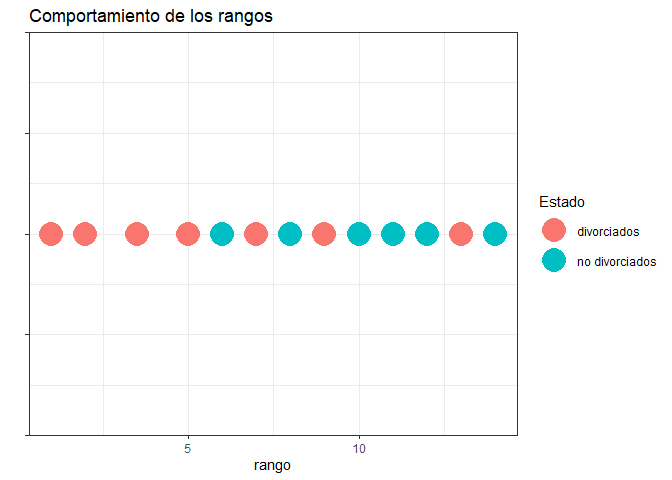
\includegraphics{Pruebas_p_files/figure-html/unnamed-chunk-87-1.png}

Procedemos a calcular \(U_{1}, \ U_{2}\).
\[U_{1}= n_{1} \ n_{2} + \frac{n_{1} (n_{1}-1)}{2} - R_{1}\]
\[U_{2}= n_{1} \ n_{2} + \frac{n_{2} (n_{2}-1)}{2} - R_{2}\] Recordamos
que \(n_{1}=n_{2}\), entonces el factor al que se le debe restar
\(R_{1}, \  R_{2}\) es el mismo.

\begin{Shaded}
\begin{Highlighting}[]
\NormalTok{factor\_us}\OtherTok{=}\NormalTok{ n\_tamanio\_muestra}\SpecialCharTok{*}\NormalTok{n\_tamanio\_muestra}\SpecialCharTok{+}\NormalTok{(n\_tamanio\_muestra}\SpecialCharTok{*}\NormalTok{(n\_tamanio\_muestra}\SpecialCharTok{+}\DecValTok{1}\NormalTok{))}\SpecialCharTok{/}\DecValTok{2}
\end{Highlighting}
\end{Shaded}

Calculamos \(U_{1}, \ U_{2}\).

\begin{Shaded}
\begin{Highlighting}[]
\NormalTok{U\_div}\OtherTok{=}\NormalTok{factor\_us }\SpecialCharTok{{-}}\NormalTok{ rango\_div}
\NormalTok{U\_nd}\OtherTok{=}\NormalTok{factor\_us }\SpecialCharTok{{-}}\NormalTok{ rango\_nodiv}
\FunctionTok{print}\NormalTok{(U\_div)}
\end{Highlighting}
\end{Shaded}

\begin{verbatim}
## [1] 36.5
\end{verbatim}

\begin{Shaded}
\begin{Highlighting}[]
\FunctionTok{print}\NormalTok{(U\_nd)}
\end{Highlighting}
\end{Shaded}

\begin{verbatim}
## [1] 12.5
\end{verbatim}

Recordamos que \(U=\min(U_{1},U_{2} )\).

\begin{Shaded}
\begin{Highlighting}[]
\NormalTok{U\_est}\OtherTok{=} \FunctionTok{min}\NormalTok{(U\_div,U\_nd)}
\end{Highlighting}
\end{Shaded}

Como suponemos que los datos vienen de la distribucion normal,
obtengamos la esperanza y varianza de \(U\), que ser??n los par??metros
para la distribucion normal, como se sugiere en las notas.

\[E[U]= \frac{n_{1}n_{2} }{2}\]
\[Var[U] = \frac{n_{1}n_{2}}{12}(n_{1}+n_{2}+1) \]

\begin{Shaded}
\begin{Highlighting}[]
\NormalTok{mu\_div }\OtherTok{=}\NormalTok{ (n\_tamanio\_muestra}\SpecialCharTok{\^{}}\DecValTok{2}\NormalTok{)}\SpecialCharTok{/}\DecValTok{2}
\NormalTok{sigma\_div }\OtherTok{=}\NormalTok{ (n\_tamanio\_muestra}\SpecialCharTok{\^{}}\DecValTok{2} \SpecialCharTok{/} \DecValTok{12}\NormalTok{ )}\SpecialCharTok{*}\NormalTok{(n\_tamanio\_muestra}\SpecialCharTok{+}\NormalTok{n\_tamanio\_muestra}\SpecialCharTok{+}\DecValTok{1}\NormalTok{)}
\end{Highlighting}
\end{Shaded}

Por ser una prueba de dos colas para \$\alpha= 0.05 \$ tenemos que ver
que pasa con los cuantiles \(\frac{\alpha}{2}, \ 1-\frac{\alpha}{2}\),
recordamos que la distribuci??n normal es simetrica.

\begin{Shaded}
\begin{Highlighting}[]
\NormalTok{alpha\_div }\OtherTok{=} \FloatTok{0.05}
\NormalTok{z\_izq}\OtherTok{=}\FunctionTok{qnorm}\NormalTok{(alpha\_div}\SpecialCharTok{/}\DecValTok{2}\NormalTok{,}\AttributeTok{mean=}\NormalTok{mu\_div,}\AttributeTok{sd=}\FunctionTok{sqrt}\NormalTok{(sigma\_div))}
\NormalTok{z\_der}\OtherTok{=}\FunctionTok{qnorm}\NormalTok{(}\DecValTok{1}\SpecialCharTok{{-}}\NormalTok{alpha\_div}\SpecialCharTok{/}\DecValTok{2}\NormalTok{,}\AttributeTok{mean=}\NormalTok{mu\_div,}\AttributeTok{sd=}\FunctionTok{sqrt}\NormalTok{(sigma\_div))}
\FunctionTok{print}\NormalTok{(z\_izq)}
\end{Highlighting}
\end{Shaded}

\begin{verbatim}
## [1] 9.160856
\end{verbatim}

\begin{Shaded}
\begin{Highlighting}[]
\FunctionTok{print}\NormalTok{(z\_der)}
\end{Highlighting}
\end{Shaded}

\begin{verbatim}
## [1] 39.83914
\end{verbatim}

Rechazamos \(H_{0}\), si \(U< Z_{\alpha}\) o
\(U> Z_{1-\frac{\alpha}{2}}\).

\begin{Shaded}
\begin{Highlighting}[]
\NormalTok{Rechazamos\_H0\_div}\OtherTok{=}\NormalTok{(U\_est }\SpecialCharTok{\textless{}}\NormalTok{ z\_izq }\SpecialCharTok{||}\NormalTok{ U\_est }\SpecialCharTok{\textgreater{}}\NormalTok{ z\_der)}
\FunctionTok{print}\NormalTok{(Rechazamos\_H0\_div)}
\end{Highlighting}
\end{Shaded}

\begin{verbatim}
## [1] FALSE
\end{verbatim}

Por lo anterior aceptamos \(H_{0}\), entonces los datos vienen de la
misma poblaci??n.~No hay una diferencia en el aprovechamiento de los
ni??os, con un \(\alpha=0.05\) de confianza.

Para comprobar lo anterior tenemos que ver la prueba de paqueteria
nortest.

\begin{Shaded}
\begin{Highlighting}[]
\NormalTok{prueba\_wilcox }\OtherTok{=} \FunctionTok{wilcox.test}\NormalTok{(divorciados, nodivorciados, }\AttributeTok{paired=}\ConstantTok{FALSE}\NormalTok{)}
\end{Highlighting}
\end{Shaded}

\begin{verbatim}
## Warning in wilcox.test.default(divorciados, nodivorciados, paired = FALSE):
## cannot compute exact p-value with ties
\end{verbatim}

\begin{Shaded}
\begin{Highlighting}[]
\FunctionTok{print}\NormalTok{(prueba\_wilcox}\SpecialCharTok{$}\NormalTok{p.value)}
\end{Highlighting}
\end{Shaded}

\begin{verbatim}
## [1] 0.1412821
\end{verbatim}

Como el \(p-value>0.05\) aceptamos \(H_{0}\), entonces las muestras
vienen de la misma poblacion.

\hypertarget{pruebas-de-correlacion-de-rango}{%
\subsection{Pruebas de correlacion de
rango}\label{pruebas-de-correlacion-de-rango}}

\hypertarget{problema-3-1}{%
\subsection{Problema 3}\label{problema-3-1}}

La tabla que se proporciona a continuacion da el nC:mero de premios de
postgraduados en ciencia medica y la razon de muerte por millon de
tuberculosis para 1959-69.

Demuestre que estos datos muestran una fuerte evidencia de correlacion
negativa entre el numero de premios y la tasa de muerte por
tuberculosis. Explique este resultado. Use \(\alpha=0.05\).

Primero veamos los datos en un data frame.

\begin{Shaded}
\begin{Highlighting}[]
\NormalTok{tasa\_muerte}\OtherTok{\textless{}{-}}\FunctionTok{c}\NormalTok{(}\DecValTok{83}\NormalTok{,}\DecValTok{74}\NormalTok{,}\DecValTok{71}\NormalTok{,}\DecValTok{65}\NormalTok{,}\DecValTok{62}\NormalTok{,}\DecValTok{52}\NormalTok{,}\DecValTok{47}\NormalTok{,}\DecValTok{48}\NormalTok{,}\DecValTok{42}\NormalTok{,}\DecValTok{43}\NormalTok{,}\DecValTok{38}\NormalTok{)}
\NormalTok{anio}\OtherTok{\textless{}{-}}\FunctionTok{c}\NormalTok{(}\DecValTok{1959}\NormalTok{,}\DecValTok{1960}\NormalTok{,}\DecValTok{1961}\NormalTok{,}\DecValTok{1962}\NormalTok{,}\DecValTok{1963}\NormalTok{,}\DecValTok{1964}\NormalTok{,}\DecValTok{1965}\NormalTok{,}\DecValTok{1966}\NormalTok{,}\DecValTok{1967}\NormalTok{,}\DecValTok{1968}\NormalTok{,}\DecValTok{1969}\NormalTok{) }
\NormalTok{premios}\OtherTok{\textless{}{-}}\FunctionTok{c}\NormalTok{(}\DecValTok{277}\NormalTok{,}\DecValTok{318}\NormalTok{,}\DecValTok{382}\NormalTok{,}\DecValTok{441}\NormalTok{,}\DecValTok{486}\NormalTok{,}\DecValTok{597}\NormalTok{,}\DecValTok{750}\NormalTok{,}\DecValTok{738}\NormalTok{,}\DecValTok{849}\NormalTok{,}\DecValTok{932}\NormalTok{,}\DecValTok{976}\NormalTok{)}
\NormalTok{Datos\_tuber}\OtherTok{\textless{}{-}}\FunctionTok{data.frame}\NormalTok{(anio,premios,tasa\_muerte)}
\FunctionTok{print}\NormalTok{(Datos\_tuber)}
\end{Highlighting}
\end{Shaded}

\begin{verbatim}
##    anio premios tasa_muerte
## 1  1959     277          83
## 2  1960     318          74
## 3  1961     382          71
## 4  1962     441          65
## 5  1963     486          62
## 6  1964     597          52
## 7  1965     750          47
## 8  1966     738          48
## 9  1967     849          42
## 10 1968     932          43
## 11 1969     976          38
\end{verbatim}

Queremos ver si se tiene una correlacion negativa (es una prueba tipo
B), entonces proponemos la prueba de hipotesis:

\(H_{0}\): \(\rho ???0\) VS \(H_{a}\): \(\rho>0\)

\hypertarget{pruebas-de-correlacion-de-rango-1}{%
\subsection{Pruebas de correlacion de
rango}\label{pruebas-de-correlacion-de-rango-1}}

\hypertarget{problema-4-1}{%
\subsection{Problema 4}\label{problema-4-1}}

\end{document}
